\chapter{TTL and multiplexer}
In this session we first measured the latancy between the input and output signal, then we used a NOT gate with open collector to turn on a LED, thirdly we designed and built an half dulpex with two 3state gates and lastly we projected and implemented a multiplex depultiplex system with 4 signals and two bit of selection.

\section{Materials}
\begin{itemize}
\item A resistor
\item A LED
\item Power supply RIGOL DP831A
\item Waveform generator RIGOL DG1032
\item Multimeter RIGOL DM3068
\item 74LS00
\item 74LS05
\item 74LS04
\item 74LS125
\end{itemize}

\section{Experimental setup}
For measuring the time propagation of the signal in the 7400 we used the configuration in figure \ref{latency}. As input we used a square-wave with 0-5 V voltage and the frequency of 100kHz.
\begin{figure}[H]
\centering
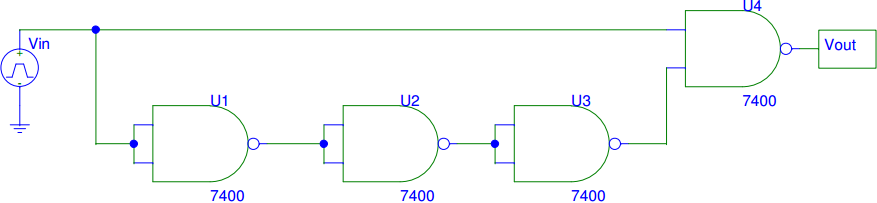
\includegraphics[width=.7\textwidth]{10/latency.png}
\caption{The circuit used for measuring the latency in the propagation of a digital input}\label{latency}
\end{figure}

For switching on and off the LED we used the circuit in \ref{LED_ON_OFF} with a power supply of 9 V and a resistor 1  k $\Omega$.
\begin{figure}[H]
\centering
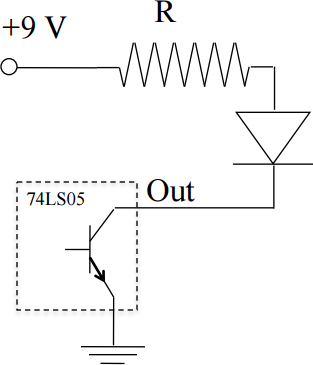
\includegraphics[width=.7\textwidth]{10/LED_ON_OFF.png}
\caption{NOT TTL Open Collector}\label{LED_ON_OFF}
\end{figure}

\\
For the half duplex we built it as in figure XX, we connected the two input by first passing the signals into a  3state that had the enable bits opposite to one another, so they passed just one singal at the time. It was possible to change signal by changing the voltage in S.
\begin{figure}[H]
\centering
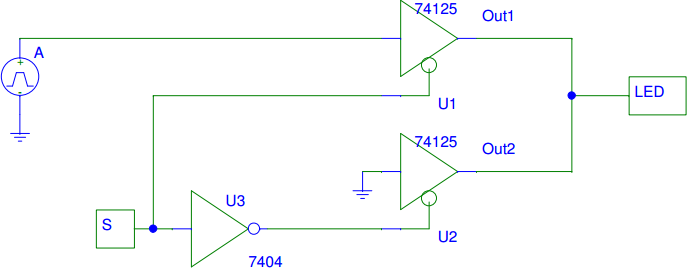
\includegraphics[width=.7\textwidth]{10/TTL_3state.png}
\caption{Half duplex used for sharing a transmission channel}\label{TTL_3state}
\end{figure}

\\
Lastly we designed a network to pass 4 different signals to all of our friends, we called this network  ``Canteriphone''. First we needed to design a multiplexer to choose between the 4 signals with 2 bits, this was implemented with the circuit \ref{multi_select}.
\begin{figure}[H]
\centering
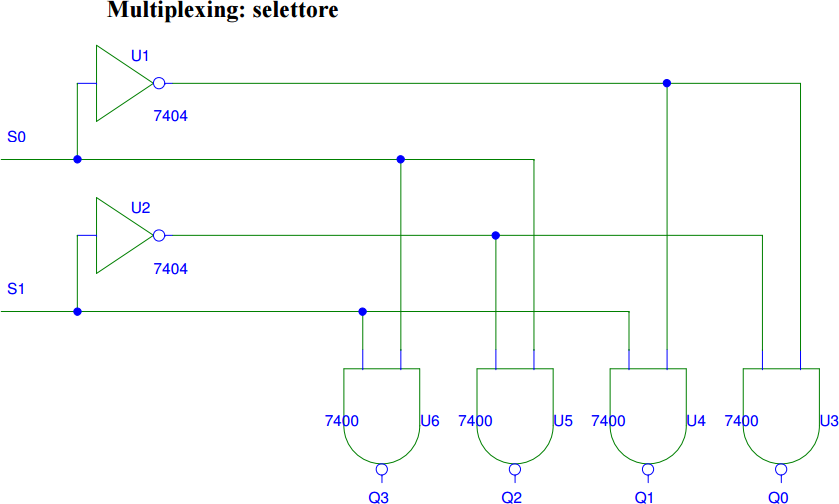
\includegraphics[width=.7\textwidth]{10/multi_select.png}
\caption{The multiplexer used for select one of the four channel}\label{multi_select}
\end{figure}

Then we used the signals from the multiplexer to enable and disable 4 3state gates that were connected with the information that we wanted to transmit, this was done in a fashon similar to the half duplex and we can see the circuit in \ref{multi_wired}.
\begin{figure}[H]
\centering
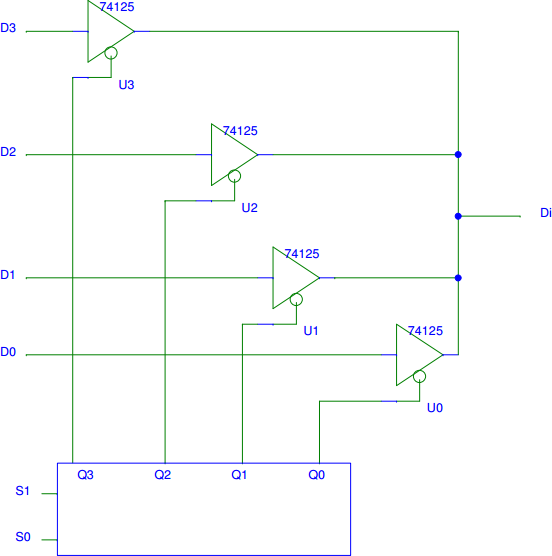
\includegraphics[width=.7\textwidth]{10/multi_wired.png}
\caption{The signal from the multiplexer used for blocking and allowing the chosen channel}\label{multi_wired}
\end{figure}

Then we took the signal from the output of the 3state gates and connected it with our friends with a cable, we also transmitted the two bits that were used to choose the signal, for allowing them to know what channel we were transmitting. Our friends built a multiplexer in \ref{multi_select} themself and used the outputs from the multiplexer and the signal transmitted to light a led with the circuit \ref{demulti}.
\begin{figure}[H]
\centering
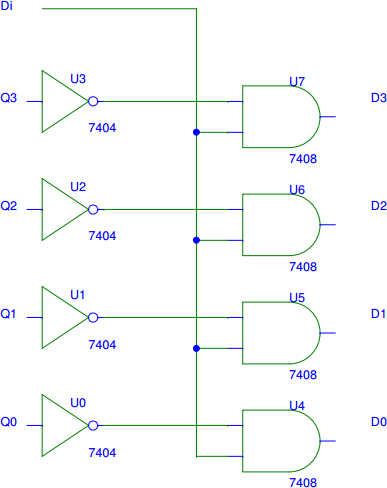
\includegraphics[width=.7\textwidth]{10/demulti.png}
\caption{De-multiplexer}\label{demulti}
\end{figure}


\section{Data analysis}
In the plot \ref{latency_plot} we can evaluate the time delay caused by the single gate. We see that the signal from the point it started descending to the point it started going up, it took about 14 ns, that divided by the three gates gives about 4.7 ns per gate. We chose the starting point when the output has a degative derivative, because that is the moment when the first pin recives the signal, and we chose the ending time when the signal invertes direction, bacause that is when the second signal propagated in all the three gates.
\begin{figure}[H]
\centering
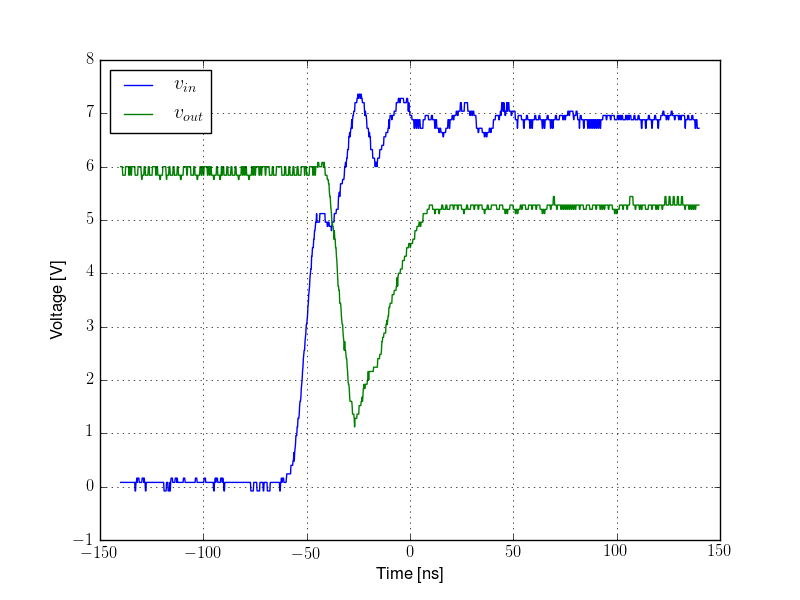
\includegraphics[width=.7\textwidth]{10/latency_plot.png}
\caption{The plot shows the delay caused by the propagation of the signal in 3 gates}\label{latency_plot}
\end{figure}
